\chapter{Connexité}


\begin{tcolorbox}
    \textbf{Connexité} : Mon espace est-il en un seul morceau ?
      \begin{figure}[H] %h:当前位置, t:顶部, b:底部, p:浮动页
        \centering
        \includegraphics[width=0.8\textwidth]{./assets/Connexité.png}
        \caption{Connexité}
        \label{fig:Connexité}
      \end{figure}

      
      \begin{itemize}
        \item \textbf{Connexité par arcs} $\implies$ Connexité
        \item Composante Connexe
      \end{itemize}


\end{tcolorbox}

\begin{tcolorbox}
    
\begin{itemize}

    \item Définitions (mémoriser par coeur)

      \begin{enumerate}

          \item Connexe par arcs, connexe
          \item Composante connexe par arcs, composante connexe 

      \end{enumerate}

    \item Théorèmes, propositions, propriétés (savoir à démontrer)
      \begin{enumerate}

          \item Image d’un connexe par arcs par une application continue 
          \item Un connexe par arc est connexe 
          \item Image d’un connexe par une application continue 
          \item Relation d’équivalence induit une partition d’espace

      \end{enumerate}

\end{itemize}
\end{tcolorbox}

\newpage
\section{Connexité par arcs}

\subsection{Chemin} % (fold)

% subsection  (end)
\begin{Definition}[colbacktitle=red!75!black]{Chemin, relié}{}
  Soit $(x,y)$ deux points de $(E,d)$, on dit $x$ est \textbf{relié à} $y$ dans $E$, s'il existe un \textbf{chemin}, qui est une application $p$ suffit :
\begin{itemize}

  \item $p:[0,1]\to E$ continue
  \item allant de $x$ à $y$, c'est-à-dire $p(0)=x,\; p(1)=y$

\end{itemize}
\end{Definition}

\subsection{Connexité par arcs} % (fold)
\label{sub:Connexité par arcs}

% subsection Connexité par arcs (end)
\begin{Definition}[colbacktitle=red!75!black]{Connexe par arc}{}
Soit $A \subset (E,d)$. On dit que $A$ est \textbf{connexe par arc}, si pour $\forall (x,y) \in A^2$, il existe un \textbf{chemin} de $x$ à $y$ \textit{dans $A$}.
\[
    \forall (x,y) \in A^2,\; \exists p \in \mathscr{C}([0,1], A),\; p(0) = x,\; p(1) = y
\]

\end{Definition}
\begin{figure}[H] %h:当前位置, t:顶部, b:底部, p:浮动页
    \centering
    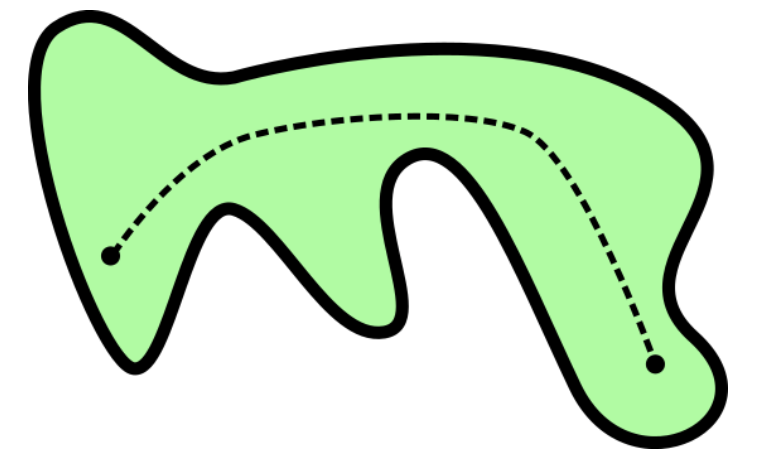
\includegraphics[width=0.3\textwidth]{./assets/Connexe par arc.png}
    \caption{Connexe par arc}
    \label{fig:Connexe-par-arc}
\end{figure}

\begin{Example}{Dans $\mathbb{R}$}{} \label{ex1}
Les connexes par arcs de $\mathbb{R}$ sont les intervalles.
\end{Example}

\begin{Example}{$\mathrm{GL} _n(\mathbb{R} )$ et $\mathrm{GL} _n(\mathbb{C})$}{}
\begin{itemize}
    \item $\mathrm{GL} _n(\mathbb{R} )$ n'est pas connexe par arc, mais $\mathrm{GL}_n ^+(\mathbb{R})$ et $\mathrm{GL}_n ^ - ( \mathbb{R})$ le sont.
    \item $\mathrm{GL} _n(\mathbb{C} )$ est connexe par arc.
\end{itemize}
\end{Example}

\begin{myproof} 
\begin{itemize}
    \item $n=1$, $\mathrm{GL}_1 (\mathbb{C} ) = [a] ,\; a\ne 0, \; a \in \mathbb{C}$.

        C'est donc à peu près $\mathbb{C} ^{*}$, qu'on visualise comme $\mathbb{R} ^{2}\backslash \{(0,0)\}$.
        \begin{center}
            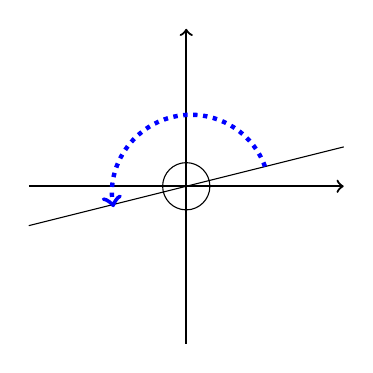
\begin{tikzpicture}
            %\node (name) at (pos1, pos2) [label={text1}] {text2};
            %\draw [option] ...;
                \draw [thick, ->] (-2,0)--(2,0);
                \draw [thick, ->] (0,-2)--(0,2);
                \draw (-2,-0.5)--(2,0.5);
                \draw (0,0) circle (.3);
                \draw [ultra thick, blue, dotted, ->] (1,0.25) arc (20:190:1);
            \end{tikzpicture}
        \end{center}
    \item
        Rappel : Algorithme du pivot du Gauss, transvection, dilatation

        Soit $A \in \mathrm{M} _n(\mathbb{C} )$ , $\mathrm{rg} (A) = r \in [\![0,n]\!]$, il existe $T_1,\ldots,T_p$ et $T_1',\ldots,T_p'$ des transvections - dilatations - permutations tel que :
        \[
            T_1\ldots T_p.A.T_1'\ldots T_q' = J_{n,n,r} = \begin{bmatrix} I_r & 0 \\ 0 & 0  \end{bmatrix} 
        \]

        Les matrices de transvection et dilatation sont respectivement : $$T_{k,l}(\lambda) = I_n + \lambda E_{k,l} = \begin{bmatrix} 1 & 0 & \ldots \\ 0 & 1 & \ldots & \lambda &  \\ \vdots &  & \ddots\\ 0 &&  \ldots && 1\end{bmatrix}, \quad D_{k}(\lambda) = I_n + (\lambda-1) . E_{k,k} = \begin{bmatrix} 1 & 0 \\ 0 & 1 \\ \vdots & & \lambda \\ 0 & \cdots & & 1 \end{bmatrix} $$
        
    \item Ici, $A \in \mathrm{GL} _n(\mathbb{C})$, on peut alors écrire ($\lambda$ ne doit être pas nul dans $D_k(\lambda)$) 
            \[
            A = B_1 \dots B_s = \dots =\mathrm{D} _n(\mathrm{det} (A)).T(\lambda_1)\ldots T(\lambda_q)
          \]
      C'est un chemin comme : $I_n \to B_s \to B _{s-1} .B_s \to B _{s-2}.B _{s-1}. B \to \dots \to A$.

      On le montre comme on peut mettre
      \begin{itemize}

      \item une seule dilatation  $D _{k}(\mu). D _{k'}(\mu') \to \dots \to D_n(\det(A))$
          \item à gauche : $T _{k,l}(\lambda) .D_j( \mu) = D _{j'}( \mu'). T _{k'. l'}( \lambda')$

      \end{itemize}


    
            
    \item Cherchons un chemin allant de $A$ à  $I_n$ dans $\mathrm{GL} _n(\mathbb{C})$
    On construit, en sachant que $M = \mathrm{D}_n(1).M$ :
    \begin{align*}
        \gamma _1 : [0,1] &\to \mathrm{GL} _n(\mathbb{C} ) \\
        t &\mapsto T_{kl}(\lambda).M
    \end{align*}
    et
    \begin{align*}
        \gamma _2 : [0,1] &\to \mathrm{GL} _n(\mathbb{C} ) \\
        t &\mapsto \mathrm{D} _n (1+t(\mathrm{det} (A)-1)).M = \mathrm{D}_n \psi (t) M 
    \end{align*}
    avec $$\psi : t \mapsto 1 + t(\det(A)-1)$$ suffit $\psi(0)=1$,  $\psi(1)= \mathrm{det} (A)$, et $1 / (\mathrm{det} (A)-1) \in [0,1]$

    Dans $\mathrm{GL} _n(\mathbb{C})$ on peut trouver une chemin canonique de $1$ à $\det A$, mais dans  $\mathrm{GL} _n(\mathbb{R} )$, par exemple on ne pourra pas aller de 1 à -1.

    Quand on passe de $A$ à $B$, $\phi$ a une restriction :  $\det(A)$ et $\det(B)$ ne doivent pas avoir des signes opposés. Donc $\mathrm{GL} _n(\mathbb{R} )$ a deux morceaux, respectivement $\det (A) >0$ et  $\det(A)<0$.
\end{itemize}
\end{myproof}

\begin{Example}{Dans espace vectoriel normé}{}
    \begin{itemize}
        \item Les convexes d'un espace vectoriel normé sont \textbf{connexe par arc} 
            \begin{center}
                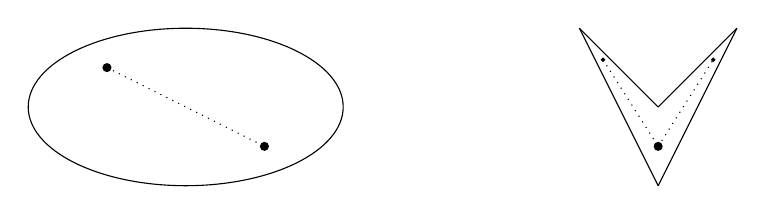
\begin{tikzpicture}
                %\node (name) at (pos1, pos2) [label={text1}] {text2};
                %\draw [option] ...;
                \draw (0,0) ellipse (2 and 1);
                \filldraw (-1,0.5) circle (.05);
                \filldraw (1,-0.5) circle (.05);
                \draw [dotted] (-1,0.5)--(1,-0.5);
                \draw (5,1)--(6,-1);
                \draw (5,1)--(6,0);
                \draw (6,0)--(7,1);
                \draw (6,-1)--(7,1);
                \filldraw (6,-0.5) circle (.05);
                \filldraw (5.3,0.6) circle (.02);
                \filldraw (6.7,0.6) circle (.02);
                \draw [dotted] (5.3,0.6)--(6,-0.5);
                \draw [dotted] (6,-0.5)--(6.7,0.6);
                \end{tikzpicture}
            \end{center}
        \item Les étoilés d'un espace vectoriel normé sont \textbf{connexe par arc}
    \end{itemize}
\end{Example}

\begin{myproof}
\begin{enumerate}
    \item $E$ convexe  $\iff$ $\forall (x,y) \in E^{2}, \forall t \in [0,1], \; tx+(1-t)y \in E$.

    Soit $(x,y) \in E^{2}$. On pose :
    \begin{align*}
        \varphi : [0, 1] &\to E \\
        t &\mapsto tx+(1-t)y
    \end{align*}

    est un chemin de $x$ à $y$ dans $E$. ($\varphi(0)=y,\; \varphi(1)=x$,  $\varphi$ est continue)
   Donc, $E$ est connexe par arcs

\item $E$ étoilé $\iff$ $\exists x_0 \in E$, $\forall  y \in E$, $\forall t \in [0,1]$, $tx_0 + (1-t)y \in E$.

    Soit $(x,y)\in E^{2}$, $[x, x_0] \subset E$ et $[x_0, y] \subset E$, on pose :
    \begin{align*}
        \varphi : [0,1] &\to E \\
        t &\mapsto \begin{cases}
            2tx_0 + (1-2t)x \text{ si } t \in [0, \frac{1}{2} ] \\
            2 \overline{t} y + (1- 2 \overline{t}) x_0 \text{ avec } \overline{t} = t - \frac{1}{2} \text{ si } t \in [\frac{1}{2} , 1]
        \end{cases}
    \end{align*}
    $\varphi$ est continue, $\varphi(0)=x$ et  $\varphi(1)=y$ donc  $\varphi$ est un chemin de $x$ à  $y$ dans $E$, $E$ est connexe par arc.
\end{enumerate}
\end{myproof}
\begin{Prop}{Image d'un connexe par arcs par une application continue}{}
Soit $E$ est \textbf{connexe par arc}, $E'$ est un espace métrique.  $f:E \mapsto E'$ une fonction continue. Donc,
\center
$f(E)$ est \textbf{connexe par arc}
\end{Prop}

\begin{myproof}{}{}
Soit $(x', y') \in f(E) ^{2}$, alors il exist $(x, y)\in E ^{2}$ tel que $x'= f(x)$ et $y'=f(y)$. 

Comme $E$ est connexe par arc, il existe $p$ allant de $x$ à $y$ dans $E$. De plus, comme $f$ est continue, $f \circ p$ est un chemin allant de $x'= f(x)$ à $y'=f(y)$ dans $f(E)$.
\end{myproof}


\begin{Example}{Homéomorphisme de deux espace}{}
$\mathbb{R} $ et $\mathbb{R} ^{2}$ ne sont pas homéomorphes. (Homéomorphes - Existe-il une \underline{bijection} $\psi:E\to F$ suffit à la fois elle-même est \underline{continue} et $\psi^{-1}$ est \underline{continue} ?)
\end{Example}

\begin{myproof}
  \begin{itemize}

      \item Si $\phi$ est un homéomrphe de  $\mathbb{R} ^{2}$ à $\mathbb{R}$, alors $\overline{\phi}: \mathbb{R} ^{2}\backslash \{(0,0)\} \to \mathbb{R} \backslash \{\phi((0,0))\}$ seraient homéomorphe. 

      \item Le premier est connexe par arc, mais la deuxième ne l'est pas. 

      \item Contradiction de la proposition précédant.

  \end{itemize}
\end{myproof}


\subsection{Composante connexe par arcs} % (fold)
\label{sub:Composante connexe par arcs}

\begin{Prop}{$x$ relié à $y$ est une relation d'équivalence}{}
Soit $A \subset (E,d)$, on définit une relation $\mathcal{R}$ sur $A \times  A$ :
\[
    \forall (x,y) \in A^2, x \mathcal{R}  y = [x \text{ relié à } y]
\]
Donc, $\mathcal{R} $ est une \textbf{relation d'équivalence}. (symétrique, réflexive, transitive)
\begin{align*}
    x &\mathcal{R}  x \\
    x \mathcal{R}  y &= y \mathcal{R}  x \\
    x \mathcal{R} y, \; y \mathcal{R} z &\implies x \mathcal{R} z
\end{align*}
\end{Prop}

\begin{myproof}
Soit $x,y$ 2 points de $A$.
\begin{itemize}
    \item $x \mapsto x$ la fonction constante.
    \item Soit $\gamma: [a,b] \to A$, on a $\bar \gamma : t \mapsto \gamma(a+b-t)$
    \item Il existe un chemin $\gamma_1$ reliant $x$ à $y$ dans  $A$, et un chemin $\gamma_2$ reliant $y$ à  $z$ dans  $A$.  $\gamma_1:[0,1] \to A$, $\gamma_2:[1,2]\to A$, on considère le chemin :
        \[
        \gamma : t \mapsto \gamma(t) = \begin{cases}
            \gamma_1(t) \text{ si } t \in [0,1]\\
            \gamma_2(t) \text{ si } t \in [1,2]
        \end{cases}
        \]

        $\gamma_1(1) = y = \gamma_2(0)$ continuité à gauche en 1. De même, continuité à droite en 1.
        
\end{itemize}
\end{myproof}

\begin{Definition}[colbacktitle=red!75!black]{Composante connexe par arcs}{}
Les classes d'équivalence $x \mathcal{R}y$ ou $x\in A$ sont appelées les \textbf{composantes connexes par arcs de $A$}, et forment une partition de $A$.
\end{Definition}


\begin{Definition}[colbacktitle=red!75!black]{Composante connexe par arcs de $x$ dans $A$}{}
La \textbf{composante connexe par arcs de $x$ dans $A$} est \underline{la plus grande partie connexe par arcs} de $A$ contenant $x$.
\end{Definition}

\begin{Prop}{Caractérisation des ouverts de $\mathbb{R}$}{}
Tout ouvert de $\mathbb{R}$ est réunion \underline{dénombrable} d'\underline{intervalles} \underline{ouverts} \underline{disjoints}.
\end{Prop}

\begin{myproof}{}{}
Soit $O$ un ouvert et notons $(E_i) _{i\in I}$ indexé les composantes connnexes par arcs de $O$. Alors, 
\begin{itemize}

  \item $\forall i\in I$, $E_i$ est un intervalle, car $E_i$ est connexe par arc de $\mathbb{R}$ (Voir \ref{ex1})

  \item $\forall i\in I$, $E_i$ est ouvert non vide. Soit $E_i$ ne l'est pas, supposons que $]a,b] \subset E_i$, alors $\exists \varepsilon >0$, $]b,b+\varepsilon[ \cap E_i = \emptyset$

  \item Les intervalles sont disjoints, car par définition d'une partition.

  \item $I$ est dénombrable, d'après une application injective de $I$ dans $\mathbb{Q}$ : $i \mapsto x_i \in E_i \cap \mathbb{Q} \ne \emptyset$

\end{itemize}
\end{myproof}


% subsection Composante connexe par arcs (end)

\newpage
\section{Connexité}

\subsection{Espace connexe} % (fold)
\label{sub:Espace connexe}

% subsection Espace connexe (end)
\begin{Definition}[colbacktitle=red!75!black]{Espace connexe}{}
    \begin{center}
        Un espace \textbf{connexe} est une partie en un seul morceau. 
    \end{center}

Plus précisément, soit $A \subset (E,d)$, les assertions suivant sont équivalentes :
\begin{enumerate}
    \item $A$ est un espace topologique \textbf{connexe}.
    \item Les seules parties à la fois ouvertes et fermées dans $A$ sont $A$ ou $\emptyset$
        \begin{center}
            Si $B \subset A$ ouvert et fermé de $A$, alors $B = \emptyset$ ou  $B=A$
        \end{center}
\begin{note}
La deuxième est le plus utilisé lorsque on veut montrer $A$ est connexe.

On commence par supposons qu'une sous-ensemble ouverte et fermée $B \ne \emptyset \subset A$, ensuite on prouvera $B=A$.


\end{note}
        
    \item $A$ n'est pas la réunion de deux ouverts/fermés non vides disjoints
        \begin{itemize}
            \item Pour tout $O_1$ et  $O_2$ sont ouverts \textit{disjoints} dans $A$, si $A = O_1 \cup O_2$, alors $O_1 = O_2 = \emptyset$ 
            \item Pour tout $F_1$ et  $F_2$ sont ouverts \textit{disjoints} dans $A$, si $A = F_1 \cup F_2$, alors $F_1 = F_2 = \emptyset$ 
        \end{itemize}
\end{enumerate}

\end{Definition}




\begin{Example}{}{}
    $A = \mathbb{R} ^*$ n'est pas connexe.
\end{Example}

\begin{myproof}{}{}
  \begin{itemize}
      \item $]-\infty, 0[$ est ouvert dans  $A$
      \item $]-\infty, 0[$ est fermé dans  $A$, c'est parce que  $]0, +\infty[$ est ouvert
      \item $]-\infty, 0[$ n'est pas égale à $A$ ou  $\emptyset$ 
  \end{itemize}
\end{myproof}


\begin{Example}{}{}
Dans $\mathbb{R}$, les intervalles $I$ sont connexe dans $\mathbb{R}$.
\end{Example}







\begin{myproof}
\begin{itemize}
    \item 
$I$ intervalle de $\mathbb{R}$, donc $I$ convexe, cela montre que $I$ est \textbf{connexe}.

\item Par contraposition, on montra que si  $I$ n'est pas intervalle, donc  $I$ n'est pas connexe.

Soit $A \subset \mathbb{R} $ n'est pas un intervalle, caractérisation :
$\exists (\alpha,\beta,\gamma) \in \mathbb{R}$, $\alpha < \beta < \gamma$ et $\alpha,\beta \in A$ mais $\beta \not\in A$

On pose $\mathcal{U}  = A \cap ]-\infty, \beta[$ et $\mathcal{V} =A \cap ]\beta, +\infty[$ des ouverts de $A$. (\textit{Ce n'est pas de $\mathbb{R}$})

On a 
\begin{itemize}
    \item $\mathcal{U} \cap \mathcal{V} = \emptyset$ car $]-\infty, \beta[ \cap ]\beta, +\infty[ = \emptyset$.
        \item $\mathcal{U} \cup \mathcal{V}  = (A \cap ]-\infty, \beta[) \cup (A \cap ]\beta, + \infty[) = A \cap (\mathbb{R} \backslash \{\beta\}) = A$ car $\beta \not \in A$
        \item De plus $\alpha \in \mathcal{U} $ et $\gamma \in \mathcal{V} $, donc $\mathcal{U} \ne \emptyset$ et $\mathcal{V} \ne \emptyset$
\end{itemize}
Alors $A$ n'est pas connexe.

Donc les connexe de $\mathbb{R}$ sont bien des intervalles.
\end{itemize}
\end{myproof}



\begin{Prop}{Image d'un connexe par une application continue}{}
Soit $(E,d)$ un espace \textbf{connexe}, $f: E \to E'$ continue. Donc,
\begin{center}
    $f(E)$ est \textbf{connexe}
\end{center}
\end{Prop}

\begin{myproof}
Soit $B \ne \emptyset$,  $B \subset f(E)$, $B$ est ouvert et fermé dans $(E',d)$, montrer que  $B = f(E)$
 \begin{itemize}
     \item $f^{-1}(B)$ est un ouvert de $E$
     \item  $f^{-1}(B)$ est un fermé de $E$
     \item  $f^{-1}(B) \ne \emptyset$ car $B \ne \emptyset$ et  $B \subset f(E) \to f^{-1}(B)=E$, donc $B = f(E)$
\end{itemize}
\end{myproof}

\begin{Example}{Théorème des valeurs intermédiaires}{}
Soit $A\subset (E,d)$ un connexe. Soit $f:A \to \mathbb{R}$ une application continue sur $A$ telle qu'il existe $(x,y)\in A^2$ vérifiant $f(x)<0$ et $f(y)>0$. Donc $f$ s'annule en un point.
\end{Example}

\begin{myproof}
D'après la proposition, $f(A)$ est un connexe de $\mathbb{R}$, donc un intervalle.

$0 \in [f(x), f(y)] \subset f(A)$, c'est-à-dire $\exists x_0 \in A$, $f(x_0)=0$
\end{myproof}


\begin{Prop}{Une autre méthode pour prouver que $A$ soit connexe}{}
$A \subset (E,d)$ est topologique \textbf{connexe} si et seulement si toute application continue $f : A \to \mathbb{Z} $ est constante.

On remplace parfois $\mathbb{Z}$ par deux valeurs distincts, par exemple $\{0,1\}$.
\end{Prop}

\begin{myproof} Dans deux sens :
    \begin{itemize}
        \item ($\implies$)

            Soit $x \in A$ et  $n = f(x)$. Comme  $\{n\}\in \mathbb{Z}$ est à la fois ouvert et fermé, $f$ est continue, $\emptyset \ne f^{-1}(\{n\}) \subset A$ est donc à la fois ouvert et fermé.

            Or, $A$ est connexe, cela implique que  $f^{-1}(\{n\}) = A$, et $f$ est constante (égale à $n$).

        \item ($\impliedby$)

            Soit $X = O_1 \cup O_2$ où les deux ouverts sont disjoints. On a $1_{O_1}: A \to \mathbb{Z} $ à la fois constant et continue, comme $1$ est ouvert et $O_1$ est ouvert.

            Ainsi, ou bien  $\varphi =1$ et  $O_2 = \emptyset$, ou bien  $\varphi = 0$ et  $O_1 = \emptyset$.


    \end{itemize}
\end{myproof}

\begin{Example}{Dans $\mathbb{R}$}{}
Les connexes de $\mathbb{R}$ sont les intervalles.
\end{Example}
\begin{myproof}{}{}
Toute fonction $f'(x) = 0$,  $f$ est constante sur $I$.
\end{myproof}
\begin{Prop}{Prolongement du connexité}{}
  Soit $A$ connexe dans $E$, donc tout ensemble $B$ tel que $A \subseteq B \subseteq \overline{A}$ (ainsi que $\overline{A}$) sont tous connexes.
\end{Prop}

\begin{myproof}{}{}
  Soit $f :B \to \{0,1\}$ continue. Comme $f$ est constante sur $A$, donc $f$ est constante sur $B$ car $B \subseteq \overline{A}$
\end{myproof}

\begin{Prop}{}{}
Une réunion de connexes d'intersection non vide est connexe.
\end{Prop}






\subsection{Connexité par arc et connexité} % (fold)
\label{sub:Connexité par arc et connexité}

% subsection Connexité par arc et Connexité (end)
\begin{Prop}{Relation entre connexe par arc et connexe}{}
\begin{center}
    Connexe par arc $\implies$ Connexe. La réciproque est fausse en générale.
\end{center}
\end{Prop}

\begin{note}
\begin{itemize}
    \item La connexité par arcs est une notion facile.
    \item La connexité est une notion un peu difficile.
\end{itemize}

Donc, toujours essayer d'utiliser la connexité par arcs : Connexe par arcs $\implies$ connexe
\end{note}
\begin{myproof}
Soit $C$ \textbf{connexe par arc}, et $B$ ouvert et fermé et non vide de $C$.
\begin{figure}[H] %h:当前位置, t:顶部, b:底部, p:浮动页
    \centering
    \includegraphics[width=0.8\textwidth]{./assets/De connexe par arc à connexe.png}
    \caption{De connexe par arc à connexe}
    \label{fig:De-connexe-par-arc-à-connexe}
\end{figure}

Soit $\varphi:[0,1]\to C$ un chemin reliant $x$ à $y$ dans  $C$.

Si  $B \ne C$, on trouve  $x \in B$,  $y \in B^{c}$.
$\Delta = \{t \in [0,1], \varphi(t) \in B\}$ et $\sup \Delta = \delta$,  $\varphi(\delta) \in B$ car  $\varphi$ continue et \underline{$B$ fermé dans $C$}.

De plus, \underline{$B$ ouvert dans $C$}, donc il existe $r >0$, $BO_C(\varphi(\delta),r)\subset B$.

Si $\varepsilon >0$ assez petit et $\delta \ne 1$, $\varphi(\delta+\varepsilon) \in B$ d'après la continuité de  $\varphi$.

Cela montre que $\delta+ \varepsilon \in \Delta$, contradit la définition de  $\delta = \sup (\Delta)$

Conclusion : Il est impossible de trouver  $x\in B$ et  $y \not\in B$ dans  $C$.

Donc,  $B=C$.
\end{myproof}


\begin{Example}{Connexe non connexe par arcs}{}
    $$A = \left\{\left(x, \sin\left(\frac{1}{x} \right)\right), x\in \mathbb{R} ^{*}\right\}\bigcup \{0\} \times [-1,1]$$ (adhérence du premier terme) est connexe, mais pas connexe par arcs.
\end{Example}

\begin{myproof}
    On note $A = C_1 \cup C_2 \cup C_3$ avec
    \begin{align*}
        C_1 &= \{(x,\sin(1 / x)), x>0\}\\
        C_2 &= \{(x,\sin(1 / x)), x<0\}\\
        C_3 &= \{0\} \times [-1,1]
    \end{align*}
    
Soit $B \subset A$, $B \ne \emptyset$ ouvert et fermé.
\begin{itemize}
    \item $C_1$, $C_2$ et $C_3$ sont tous connexes par arcs.
    \item Rappel : $O$ (resp. $F$) ouvert (resp. fermé) de $(E, d)$, si $A \subset E$, $A \cap O$ (resp. $A \cap E$) ouvert (resp. fermé) de $A$.
    \item Montrer que $B=A$.
        \begin{itemize}
            \item Soit $B \cap C_1 \ne \emptyset$, alors $B \cap C_1$ est ouvert et fermé dans $C_1$ car $B$ est ouvert et fermé dans $A$.

            En outre, $B\ne \emptyset, B \cap C_1 = C_1$ car $C_1$ est connexe par arcs donc connexe.
            \item 
        De même, si $B \cap C_2 \ne \emptyset$, $B \cap C_2 = C_2$ ; Si $B \cap C_3 \ne \emptyset$, $B \cap C_3 = C_3$
    \item 
      Si $B \cap C_1 \ne \emptyset$,  $B \supset C_1$ or \underline{$B$ est fermé dans $A$}, donc :  $B \supset \overline{C_1} = C_1 \cup C_3$. Donc $C_3 \subset B$.
        \item
        Comme $C_3 \subset B$, $\{0\} \times [-1,1] \subset B$, $(0,0)\in B$. Comme \underline{$B$ ouvert dans $A$}, $\exists r>0,\; BO_A((0,0), r) \subset B$, $C_2 \cap B \ne \emptyset$,  donc $B \cap C_2 = C_2$,
     \item Finalement,
          $$A = C_1 \cup C_2 \cup C_3,  \; B \subset A, \; B = (C_1 \cap B) \cup (C_2 \cap B ) \cup (C_3\cap B) = C_1 \cup C_2 \cup C_3 =A$$
        \end{itemize}
\end{itemize}

\end{myproof}

\begin{Example}{Dans espace vectoriel normé}{}
    \begin{itemize}
        \item Les convexes d'un espace vectoriel normé sont \textbf{connexe} 
        \item Les étoilés d'un espace vectoriel normé sont \textbf{connexe}
    \end{itemize}
\end{Example}
\begin{myproof}
Connexe par arcs donc connexe.
\end{myproof}

\begin{note}{}{}
Conclusion important !
\end{note}


\subsubsection{Cas d'un espace vectoriel normé} % (fold)
\label{sec:Cas d'un espace vectoriel normé}

% subsubsection Cas d'espace vectoriel normé (end)

\begin{Theorem}{Dans espace vectoriel normé}{}
Dans un espace vectoriel normé, tout \underline{ouvert connexe} est connexe par arcs. (Équivalence)
\end{Theorem}

\begin{note}{}{}
$(E, d)$ est connexe, on veut montrer que $\Delta = \{x\in E, \mathcal{P}(x) \text{ vraie}\} = E$ : montrer que $\Delta \ne \emptyset$, $\Delta$ est fermé dans $E$, $\Delta$ est ouvert dans $E$.
\end{note}

\begin{myproof}{}{}

Soit $O$ un ouvert connexe non vide de $(E, \| . \|)$. 

Soit $x \in O$, $\Delta = \{ y \in O,\; \text{il existe un chemin reliant } x \text{ et } y \text{ dans }O\}$. Montrons que $\Delta = O$.
\begin{itemize}

    \item $\Delta \ne \emptyset$, car $x \in \Delta$. 
    \item $\Delta$ ouvert dans $O$. 
      \begin{figure}[H] %h:当前位置, t:顶部, b:底部, p:浮动页
        \centering
        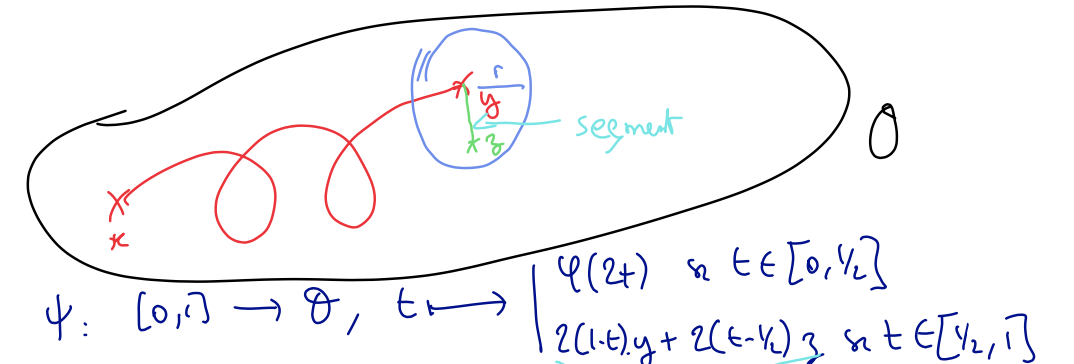
\includegraphics[width=0.9\textwidth]{./assets/Ouvert-Connexe-Pr1.png}
        \caption{Ouvert Connexe}
      \end{figure}

      Soit $y \in \Delta$, il existe $r >0$, $BO(y, r) \subset O$.

      Soit $z \in BO(y,r)$, on peut construire un chemin reliant $x$ à $z$ dans $O$. 

      Donc, $BO(y,r) \subset \Delta$.

    \item $\Delta$  fermé dans $O$.
      \begin{figure}[H] %h:当前位置, t:顶部, b:底部, p:浮动页
        \centering
        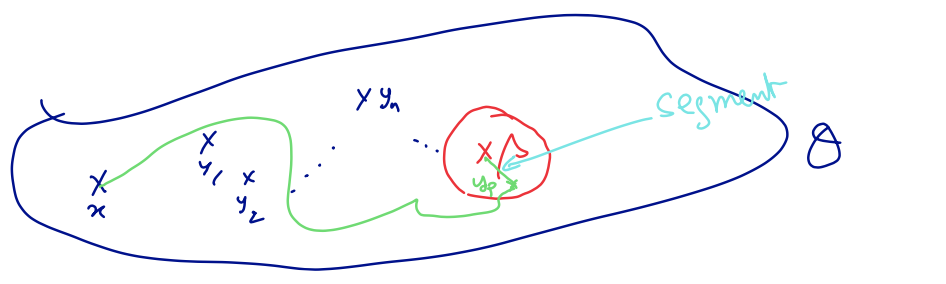
\includegraphics[width=0.9\textwidth]{./assets/Ouvert-Connexe-Pr2.png}
        \caption{Ouvert Connexe}
        \label{fig:Ouvert Connexe}
      \end{figure}

      Soit $(y_n) _{n \in \mathbb{N}} \in \Delta ^{\mathbb{N}}$ , $y_n  \underset{}{\longrightarrow} \beta \in O$. 

      Comme $O$ est ouvert, il existe $r>0$, $BO(\beta, r) \subset O$, et si $p$ assez grand, $y_p \in BO(\beta,r)$. 

      Il existe $\varphi_p$ relie $x$ à $y_p$, et le segment $[y_p, \beta]$ relie $y_p$ à $\beta$ dans $O$.

      On recolle les 2 chemins pour avoir un chemin de $x$ à $\beta$ dans $O$, donc $\beta \in \Delta$. 

\end{itemize}

En conclusion, $\Delta$ non vide, ouvert et fermé dans $O$ et $O$ connexe donc $\Delta = O$. 
\end{myproof}


\subsection{Composante connexe} % (fold)
\label{sub:Composante connexe}

% subsection Composante connexe (end)

\begin{Definition}[colbacktitle=red!75!black]{Composante connexe}{}
Soit $A \subset (E,d)$, $a \in A$, on appelle \textbf{composante connexe de $a$ dans $A$} \underline{le plus grand connexe} de $A$ contenant $a$. On la notera $C_A(a)$.
\end{Definition}

\begin{Prop}{Relation d'équivalence}{}
$\mathcal{F} = \{ C \text{ connexe } \subset A, \; a\in C\}$, suffit
\begin{itemize}

  \item $\mathcal{F } \ne \emptyset$ car $\{a\} \in \mathcal{F}$
  \item $\mathcal{F }$ stable par $\bigcup$

\end{itemize}
On obtient 
\[
  C_A(a) = \bigcup _{C \in \mathcal{F}} C
\]

La relation 
\[
  [x \mathcal{R} y ] \iff [x \in C_A(y)]
\]
induit une partition de $A$, et elle est une relation d'équivalence sur $A$. De plus, tout sous-ensemble $A$ de $E$ est réunion disjointe de ses composantes connexes.
\end{Prop}



\begin{Prop}{Sous-ensemble disjoint devient composantes connexes}{}
Soit $A \subset (E, d)$. 

$$A = \bigcup _{i \in I} C_i, \quad \forall (i,j) \in I ^{2}, \; i \ne j \implies C_i \cap C_j = \emptyset$$

Les $C_i$ sont les \textbf{composante connexe} de $A$ si :
\begin{center}
    $\forall i$, $C_i$ \underline{connexe} et $C_i$ \underline{ouverte} dans $A$
\end{center}
\end{Prop}

\begin{myproof}{}{}
Soit $a \in A$, il existe (unique) $i_0\in I$, $a \in C _{i_0}$. 
\begin{itemize}

    \item $C _{i_0}$ connexe, donc $C _{i_0} \subset C_A(a)$. (Définition : Composante connexe est le plus grand \underline{connexe} inclus dans $A$ contenant $a$)

    \item Comme $C _{A}(a) \subset A$,
      \[
        C_A(a) = \bigcup _{i \in I} \left(C_i \cap C_A(a)\right) = C _{i_0} \cup \left( \bigcup _{i \in I,\; i \ne i_0} C_i \cap C_A(a)\right)
      \]

      $C _{i_0}$ est donc fermé car $C_i \cap C_A(a)$ est ouvert dans $C_A(a)$ car $C_i$ ouvert dans $A$.


\end{itemize}

Or $C _{i_0}$ est ouvert d'après définition. Elle est aussi non nul. Comme $C_A(a)$ est connexe, $C _{i_0} = C_A(a)$
\end{myproof}






